%!TEX root = tesis.tex


\chapter{Un \ssolver paralelo y distribuido }
\label{ssolver-pardist}

La implementación de nuestra herramienta como un sistema distribuido persigue
el objetivo fundamental de mejorar el tiempo de ejecución ya sea decrementando
el tiempo necesario para resolver un problema determinado, o transformando un
problema previamente irresoluble (en tiempo razonable) en resoluble. Para ello
el sistema debe ser \textbf{escalable} en tanto que debe tener la capacidad de
sacar provecho de la incorporación una mayor cantidad de \hard a la infraestructura
utilizada en la resolución del problema. Por otro
lado, el uso de este \hard debe ser \textbf{eficiente} en el sentido de que la
utilización de mayor cantidad de \hard debe resultar en un mejora de la
performance del sistema (en nuestro caso entendida como se describió
previamente).

\begin{wrapfigure}{R}{0.4\textwidth}
\includegraphics[scale=0.4]{graphs/split por guiding path}
\caption{Esquema de partición por \gp}
\label{fig:guidingpaths}
\end{wrapfigure}

Con estos dos objetivos en mente desarrollamos una \ssolver distribuido basado
en la idea de \gp y orientado a que su utilización sea en \clusters de computadoras. La idea de \gp se
basa en la observación de que, en el peor caso, todas las posibles valuaciones
de una fórmula proposicional $\varphi$ deben ser evaluadas. Una vez que una
valuación que satisface a una fórmula es encontrada, el procedimiento de
\ssolving puede darse por finalizado\footnote{Existe otra variante en la que, además
de determinar si una fórmula es \sat o \unsat, interesa enumerar todos los
posibles modelos de dicha fórmula. En este escenario el procedimiento de
\ssolving no puede ser detenido una vez que se encuentra una valuación sino
que el mismo debe continuar hasta agotar todas las posibles valuaciones que
satisfacen a la fórmula en cuestión.}. Por el contrario, si la fórmula es
\unsat, la única alternativa para poder asegurarlo es agotar todas las
posibles valuaciones y determinar que ninguna de ellas satisface a la fórmula
en cuestión. Por lo tanto, una forma de dividir el problema es tomar una
variable $v$ y construir los dos subproblemas $\varphi_{v \leftarrow 0}$ y
$\varphi_{v \leftarrow 1}$ que se derivan de las dos posibles asignaciones de
valores de verdad a dicha variable. Una vez hecho esto, determinar que el
problema original $\varphi$ es \unsat se reduce a determinar que tanto
$\varphi_{v \leftarrow 0}$ como $\varphi_{v \leftarrow 1}$ son \unsat. Por el
contrario, determinar que el problema es \sat reduciría a establecer que
$\varphi_{v \leftarrow 0}$ es \sat o bien que $\varphi_{v \leftarrow 1}$ lo
es. Ahora, $\varphi_{v \leftarrow 0}$ y $\varphi_{v \leftarrow 1}$ pueden ser
considerados como dos problemas independientes y volver a aplicar la misma
idea recursivamente. Naturalmente este proceso puede realizarse seleccionando
más de una variable en cada paso. Al seleccionar $n$ variables obtendremos
entonces $2^n$ subproblemas. Llamaremos \emph{levantar variables} al proceso
de dividir un problema $\varphi$ en los $2^n$ subproblemas que resultan de
aplicar todas las posibles valuaciones sobre el conjunto de $n$ variables
levantadas. Se desprende de esto que una de las tareas que debe poder realizar
la herramienta es la de dividir un problema en los subproblemas que derivan de 
adoptar todos los posible \gp para un conjunto de variables.

% El objetivo principal de todo sistema distribuido es que el mismo sea
% \textbf{escalable}. Si bien la escalabilidad puede ser entendidad en
% diferentes sentidos, nos interesa en particular que el sistema haga posible la
% utilización de mayor cantida de \hard para resolver el problema (en nuestro
% caso un problema \sat) y que esa utilización de mayor poder de cómputo reporte
% ganancias en términos de tiempo (percibido) invertido en resolver un
% determinado problema o bien en términos de empujar la frontera de lo
% resoluble.

%La escalabilidad como gran objetivo rector en el desarrollo de nuestra
%herramienta introduce una serie de desafíos, a saber:
%\begin{itemize}
%	\item Almacenamiento distribuido.
%	\item Simetría de capacidades en los nodos de trabajo (\ws).
%	\item Minimización de la utilización de la red de comunicaciones.
%\end{itemize}


\section{Objetivos de diseño y desafíos asociados}

\subsection{Aspectos básicos de escalabilidad}

En primer término consideraremos los desafíos asociados con ciertos aspectos
básicos que, de no ser adecuadamente manejados, podrían atentar de modo flagrante
contra la escalabilidad de la herramienta.

\subsubsection{Almacenamiento distribuido}

La necesidad de que el almacenamiento de problemas pendientes de resolución se
encuentre distribuido se debe a un doble aspecto. Por un lado, la cantidad de
subproblemas producidos puede ser muy grande. Por lo tanto no es razonable
requerir que la cantidad de espacio necesario para almacenar todas las tareas
pendientes de resolución se encuentre disponible en una misma ubicación.

Aún si fuera posible contar con la cantidad de espacio necesaria para almacenar
todos los subproblemas en una ubicación centralizada, surge un segundo problema
que presentaría este enfoque: el de la contención de acceso a la información asociada a un problema. 
Si pretendemos que el almacenamiento no se vuelva un cuello de botella, es vital
distribuir las tareas pendientes de modo que cuando los \ws requieran nuevas
tareas para resolver, los múltiples pedidos no recaigan siempre sobre un mismo equipo.


\subsubsection{Simetría en las capacidades de los \ws}

El requisito de que los nodos de trabajo (\ws) sean simétricos también se desprende
de la necesidad de eliminar los potenciales cuellos de botella. La simetría, entendida en su
máxima expresión como la posibilidad de que todas las unidades de
procesamiento puedan realizar todas las funciones necesarias, provee la
capacidad de distribuir la carga de trabajo de la manera más conveniente en
cada momento.

Esto no podría lograrse si los nodos de trabajo tuvieran
funciones específicas, ya que podría darse el caso de tener nodos ociosos
por falta de trabajo pendiente de la clase de trabajo que esos nodos realizan, 
a la vez que otros nodos se encuentran sobrecargados. Esta situación podría empeorar
seriamente a medida que la cantidad de nodos aumenta.

En nuestro caso particular, el requisito de simetría se traduce en que
todos los \ws deben poseer las capacidades de: \begin{inparaenum}[a)] \item analizar un
subproblema hasta lograr obtener un veredicto (consumir), \item
dividir un subproblema demasiado difícil en nuevos subproblemas (producir) y \item almacenar,
solicitar y transferir subproblemas (distribuir). \end{inparaenum}


\subsubsection{Movilidad de tareas pendientes}

El triple rol de productor, consumidor y distribuidor asignado a los \ws
transforma la migración de tareas en un desafío en tanto que un \w puede
estar --y generalmente lo estará-- ocupado analizando un
subproblema cuando otro \w le solicite algún subproblema
pendiente que se encuentre en su poder.

Es claro que, ante esta situación, no sería aceptable que el \w que está
esperando una tarea se vea obligado a esperar hasta que aquel que la generó
deje de \solvear para poder acceder a la misma. Esto da origen a un requerimiento
de asincronicidad entre \emph{solving} y \emph{serving}.

Sin embargo, tampoco sería aceptable que el impacto de servir tareas bajo demanda vaya en
detrimento del análisis, que es, al fin y al cabo, el verdadero objetivo del \w.
De aquí surgen un requerimiento de sincronicidad (por ejemplo: encolar los pedidos de
tareas pendientes y atender sólo una cantidad limitada a la vez) y otro de balanceo
de carga (por ejemplo: evitar que la capacidad de almacenamiento de un \w llegue a
saturarse transfiriendo preventivamente tareas a otros \ws).

En resumen, lograr ortogonalidad entre análisis y migración de tareas es
importante para lograr escalabilidad, y sienta las bases para el desarrollo de mecanismos
avanzados de balanceo automático de carga.



\subsection{Aspectos de automatización e interactividad}

La automatización de la operatoria es un requerimiento crucial. Desde el punto
de vista del usuario, es fundamental que la herramienta sea capaz de llevar a
cabo su objetivo --demostrar la propiedad o exhibir un contraejemplo-- sin requerir
supervisión alguna ni depender de complejas parametrizaciones que requieran
numerosos experimentos para ser halladas.

Sin embargo, generar una estrategia automática que proporcione buenos resultados
en la ejecución de un amplio espectro de problemas es sumamente difícil. Desde el
punto de vista del experto que necesita diseñar, implementar, evaluar, depurar y
mejorar una estrategia no supervisada, es importante contar con alguna
interfaz interactiva que posibilite la inyección de comandos arbitrarios que permitan 
la modificación del comportamiento de la herramienta en tiempo de ejecución.

La necesidad de atender estos requerimientos encontrados motivó la adopción de
un enfoque en el que la maquinaria de cómputo distribuido (i.e. la comunidad de \ws) no posee inteligencia
propia, sino que se limita a proveer una serie de funcionalidades básicas que
pueden ser invocadas remotamente, ofreciendo un alto grado de generalidad. La
operación del sistema se lleva a cabo desde un tablero de control que permite
explorar manualmente trazas de ejecución arbitrarias. Sobre esto se monta
luego la automatización; en primer término la de aspectos reiterativos de rutina (i.e. carga de tareas al momento de la liberación de la unidad de cómputo, etc.),
y finalmente la que implementa la toma inteligente de decisiones estratégicas (i.e. cuándo es conveniente partir un problema en subproblemas, etc.).

De lo antedicho surgen tres desafíos concretos. En primer lugar, el de lograr una
arquitectura adecuada para ser totalmente controlable por un operador remoto humano.
En segundo lugar, el de diseñar las interfaces de modo tal que provean una base adecuada
para automatizar, tanto parcial como totalmente, dicho control. Y finalmente el de
diseñar e implementar la estrategia automática propiamente dicha.


\subsection{Otros aspectos de calidad}

%Además de los as de escalabilidad, surgen también los desafíos
%relacionados con la eficiencia o la performance de la herramienta. Entre ellos
%los más destacados son:
%
%\begin{itemize}
%	\item Movilidad de tareas.
%	\item Crecimiento a la par de los \ssolvers secuenciales.
%	\item No hacer burradas \todo{Revisar toda esta itemización. No me convence....}
%\end{itemize}

\subsubsection{Modularidad del componente \ssolver de los \ws}

Otro de los objetivos que perseguimos a la hora de diseñar nuestra herramienta
fue que la misma pudiera utilizar un \ssolver \ots para la resolución local de
un subproblema concentrando las tareas vinculadas al desarrollo del \ssolver en 
los aspectos de orquestación del cómputo distribuido. Esto nos permite aprovechar 
los numerosos avances logrados por
la comunidad en el área de investigación en \ssolving secuencial en los últimos
años, y a la vez nos permite, a futuro, evolucionar a la par de los \ssolvers
secuenciales, capitalizando sus nuevos logros a bajo costo y mitigando el
riesgo de que la herramienta devenga obsoleta ante un nuevo avance en dicho
campo de estudio.

\subsubsection{Mantenibilidad y modificabilidad}

El último objetivo que perseguimos durante el desarrollo de nuestra
herramienta fue que la misma presentara facilidad para ser modificada sin que
esto impactara negativamente en la \emph{performance}. Este objetivo, entre
otras cosas, determinó la elección de las tecnologías a utilizar para su
desarrollo. Por lo tanto, se utilizó el lenguaje de programación \Python para
el desarrollo de toda la herramienta con excepción de las secciones destinadas al cómputo
intensivo.

Al utilizar un \ssolver \ots no fue necesario elegir un lenguaje
para su desarrollo. En la implementación actual de la herramienta utilizamos
el \ssolver \minisatdosveinte que está desarrollado en el lenguaje \cpp. Para
ello se desarrolló un \emph{wrapper} que permite utilizar \minisat desde un
entorno \Python, obteniendo todos los beneficios de un lenguaje de programación
dinámico sin pérdida de eficiencia en los algoritmos vinculados al cómputo intensivo.

Para el intercambio de mensajes entre los \ws se utilizó el
estándar \mpi a través de la biblioteca \texttt{mpi4py}\cite{mpi4py}.


% \begin{itemize}
% 	\item Escalable
% 	\item Uso de SAT Solver off-the-shelf
% 	\item Multiplataforma
% 	\item Tablero de control
% \end{itemize}

\section{Arquitectura}

La \fig\ref{fig:arquitectura} muestra la arquitectura de la herramienta. En
la misma se distinguen claramente dos componentes: el \bend que ejecuta sobre
un \cluster de computadoras y el \fend que ejecuta en un equipo que se
encuentra posiblemente fuera del centro de cómputos.

\begin{figure}%{R}{0.45\textwidth}
\centering
\fbox{\includegraphics[scale=0.3]{graphs/paralloy architecture}}
\caption{Diagrama de componentes y conectores del \ssolver distribuido}
\label{fig:arquitectura}
\end{figure}

\subsection{\bend}
\label{sec:backend}

En el \bend se puede observar que existen dos clases distintas de elementos.
Por un lado tenemos un proceso llamado \master que es el encargado de manejar
la comunicación de órdenes desde el \fend hacia los \ws y de reenviar las
respuestas correspondientes desde los \ws hacia el \fend.

En segunda instancia encontramos otro de tipo de procesos, los \ws. Los \ws
son los encargados de relizar el cómputo (\ssolving) y la división de un
problema en nuevos subproblemas. Asimismo son quienes almacenan las tareas
pendientes de ejecución y por lo tanto deben proveer acceso a dicho
almacenamiento a los demás \ws.

Es importante destacar que si bien el \bend presenta una arquitectura
\masterslave, el \master en este caso no toma ninguna decisión sino que
simplemente actúa como intercambiador de mensajes entre el ambiente externo
(el \fend) y el ambiente interno.

\begin{figure}[h!]
\centering
\includegraphics[scale=0.4]{graphs/master proxy detail}
\caption{Detalle de arquitectura del componente \master}
\label{fig:masterproxydetail}
\end{figure}

La \fig\ref{fig:masterproxydetail} detalla la arquitectura del \master. En el
diagrama se puede observar que el \datapath de entrada (\fend hacia \bend) y
el de salida (\bend hacia \fend) son independientes. Esto es una consecuencia
directa que se desprende de la ausencia de inteligencia en el \master. Esto
implica que no es necesario mantener el estado del sistema ya que en este
componente no se toman decisiones. La ausencia de estado hace que el proceso
\master consuma un mínimo de recursos, tanto de cómputo como de almacemiento.

La intervención de dos \threads distintos en el \datapath de entrada
proporciona un alto nivel de respuesta ya que permite que algunos comandos
sean implementados internamente mediante comunicación sincrónica a través de
\mpi sin que esto implique una pausa en el procesamiento del flujo de datos de
entrada desde el \fend hacia el \bend. La comunicación sincrónica permite
simplificar algunos comandos como el envío del problema original hacia todos
los \ws. Al mismo tiempo se mantiene el orden entre los comandos enviados
desde el \fend lo cual también contribuye a la simplificación del modelo de
cómputo a pesar de tratarse de un sistema distribuido.

\begin{figure}[h!]
\centering
\includegraphics[scale=0.4]{graphs/worker detail}
\caption{Detalle de arquitectura del componente \w}
\label{fig:workerdetail}
\end{figure}

La \fig\ref{fig:workerdetail} muestra el detalle de diseño del componente
\w. Como se puede observar, las funciones de \solving, comunicación y
transferencia de archivos se implementaron en \threads separados. Dado que la
función de \solving utiliza principalmente tiempo de \cpu, mientras que el
resto de las funciones consumen principalmente tiempo de \io, la separación de
éstas en distintos \threads permite la ejecución concurrente de estas
tareas sin que esta característica impacte negativamente en el desempeño del
\ssolver. A la vez, esta característica permite satisfacer el objetivo de
movilidad de las tareas, aún cuando el \w se encuentre ocupado \solveando.

Interesa destacar también que la estrategia de partición de un problema
se encuentran implementadas en los \ws. Si
bien este diseño es contrario a la idea general basado en la existencia de un \emph{tablero de control}
consideramos que el nivel de granularidad necesario para poder controlar
remotamente la realización de estas dos tareas era demasiado alto y atentaba
contra la usabilidad de la herramienta. Asimismo, la herramienta es capaz de
poseer diversas estrategias implementadas
de modo que el usuario puede seleccionar aquella que le resulte más apropiada (y sus
parámetros en caso que corresponda) desde el \fend.

Por último, corresponde mencionar a qué nos referimos en concreto cuando
hablamos de \emph{tarea}. El término \emph{tarea} fue mencionado en varias
ocasiones a lo largo de la explicación. Si bien conceptualmente una tarea
podría ser simplemente una fórmula $\varphi$ en \cnf, en la práctica esto
podría producir un \emph{overhead} en la transferencia demasiado grande ya
que, por ejemplo al partir un problema levantando $n$ variables podríamos
generar $2^n$ subproblemas, cada uno de los cuales estaría representado
esencialmente por la misma fórmula $\varphi$ más las cláusulas unitarias
que determinan el \gp al que cada subproblema corresponde. Esta situación se repite innumerables veces a lo
largo de la ejecución de la herramienta para resolver un problema. Es por esto
que optamos, como modo de funcionamiento, por enviar la fórmula \cnf del problema original a
todos los \ws al comienzo de una ejecución de la herramienta de modo que luego
un subproblema esté representado sólo por el \gp identificado por las cláusulas unitarias necesarias para
forzar las decisiones correspondientes a ese subproblema. Esto hace que las
tareas pendientes de resolución sean mucho más económicas de manipular. 

Incluso pensando a futuro y considerando la posibilidad de implementar estrategias de
aprendizaje es necesario que, como parte de una tarea, se puedan transferir
también las cláusulas aprendidas que deban ser consideradas a los efectos de resolver esa tarea. Inclusive es
posible que en un futuro una tarea no represente únicamente un subproblema que
aún se debe intentar \solvear, sino que podría también incluir otro tipo de
actividades, como la partición de un problema. Esto último nos motivó a optar
por un concepto de tarea genérico donde una tarea no es más que un paquete de
archivos que el \w sabrá interpretar apropiadamente. En la implementación
actual las tareas son exclusivamente un subproblema pendiente de ser atacado y
se representan como un paquete con un archivo que incluye las cláusulas
unitarias que deben adicionarse al \cnf original para construir el subproblema
correspondiente más dos archivos que pueden o no contener información. Estos
últimos transportan la información de cláusulas aprendidas que deben ser
incorporados al intento de \solving del subproblema en cuestión.

\subsection{\fend}

\begin{figure}[h!]
\includegraphics[scale=0.4]{graphs/frontend architecture}
\caption{Detalle de arquitectura del \fend}
\label{fig:frontend}
\end{figure}

\begin{wrapfigure}{r}{0.6\textwidth}
	\vspace{-3em}
	\begin{subfigure}{0.27\textwidth}
		\centering
		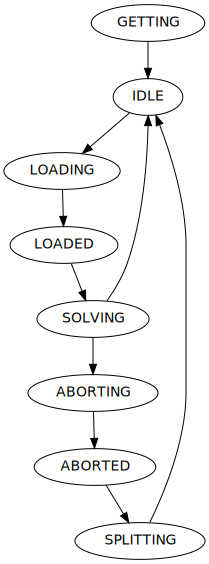
\includegraphics[scale=0.3]{graphs/workerstates}
		\caption{\emph{Workers}}
	\end{subfigure}
	\begin{subfigure}{0.27\textwidth}
		\centering
		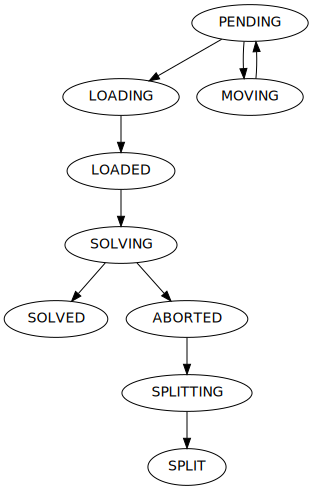
\includegraphics[scale=0.3]{graphs/taskstates}
		\caption{Tareas}
	\end{subfigure}
	\caption{Diagramas de estado en el tablero de control}
	\label{fig:states}
	\vspace{-1em}
\end{wrapfigure}

En la \fig\ref{fig:frontend} se esquematiza el diseño de componentes del
\fend. En esta figura se puede observar que el tablero de control proporciona
un modo doble de interacción con el \bend. Por un lado, el tablero de control
es capaz de recibir comandos del usuario en \rt a través de una interfaz de
tipo consola. Estos comandos representan acciones a ser llevadas a cabo en el
\bend como ser indicar a un \w ocioso que cargue una nueva tarea, indicar a un
\w que se encuentra trabajando en un problema que aborte dicha ejecución,
mover una tarea desde un \w a otro, etc. Por otro lado, el tablero de control
posee también una \emph{estrategia} (intercambiable) que permite llevar a cabo
acciones automáticamente frente a determinados eventos. El \fend posee también
un componente que procesa permanentemente la información que llega desde el
\bend. 

Es importante observar que todos los componentes mencionados comparten un
estado global. Esto se debe a que, tal como se explicó en la Sec.~\ref{sec:backend},
el \bend no tiene conocimiento del estado global del sistema. Por lo tanto, esta responsabilidad
recae en el \fend en la medida que este estado es necesario para poder tomar
decisiones ante los distintos eventos. El acceso concurrente a este estado
global nos obliga a introducir un mecanismo de sincronización entre los
distintos \threads de ejecución (\emph{locking}) que garantice la consistencia
del estado en todo momento. Hemos tenido el cuidado necesario para evitar que
el \emph{locking} atente contra la performance del componente en cuestión.

\begin{wrapfigure}{r}{.6\textwidth}
\vspace{-2em}
\begin{footnotesize}
\begin{lstlisting}[mathescape,language=Pascal,frame=single,label=lst:synchronouscmd,caption=Esquema de comando sincrónico]
DECIR_A $W$ que obtenga la tarea $T$
ESPERAR que tarea $T$ este en $W$
DECIR_A $W$ que cargue tarea $T$
ESPERAR que tarea $T$ este cargada
DECIR_A $W$ que comience a solvear $T$
\end{lstlisting}
\end{footnotesize}
\vspace{-1.5em}
\end{wrapfigure}

En la \fig\ref{fig:states} presentamos las máquinas de estado correspondientes
a los \ws y a las tareas. Estos diagramas esquematizan la información básica que
es mantenida automáticamente en el modelo del estado global del \fend. Una estrategia
particular podría requerir un estado más rico, que incluya mayores detalles, para
tomar sus decisiones. Por ejemplo, se podría requerir mantener cierta información
histórica sobre la ejecución en curso. En tal caso es responsabilidad de dicha
estrategia la implementación de las estructuras de datos y algoritmos adicionales
necesarios.


\begin{wrapfigure}{r}{.6\textwidth}
\begin{footnotesize}
\begin{lstlisting}[language=Python,caption=Interfaz Strategy,label=lst:strategy]
class Strategy(object):
	def register_globalstate(globalstate)
	def register_socket(commandsocket)
	def on_init(worker)
	def on_createroot(worker, task)
	def on_init_finished(nworkers)
	def on_getfile(worker, task)
	def on_file(worker, task)
	def on_load(worker, task)
	def on_unsat(worker, task)
	def on_sat(worker, task, modelstr)
	def on_abort(worker, task)
	def on_split_newtask(worker, newtask)
	def on_split_finished(worker, 
	                      parenttask, 
	                      nchildren)
	def on_shutdown()
\end{lstlisting}
\end{footnotesize}
\vspace{-3em}
\end{wrapfigure}

En cuanto a las estrategias, se siguió un modelo reactivo (\emph{eventos}).
Esto se debió en primera instancia a la dificultad de ejecutar secuencias de
comandos de forma sincrónica. Por ejemplo, si quisiéramos implementar la
obtención automática de una nueva tarea cuando un \w se queda sin tareas
pendientes y quisiéramos además que el \w comenzara a \solvear dicha tarea en
el momento en el que la misma esté disponible, deberíamos implementar un
algoritmo similar al expuesto en \lst\ref{lst:synchronouscmd}. El problema en
este algoritmo se encuentra en las líneas que comienzan con la palabra clave
\texttt{ESPERAR} ya que no es aceptable que la consola de comandos o la
estrategia se bloqueen a la espera de un evento que puede tardar una cantidad
arbitraria de tiempo en ocurrir. Esto se debe principalmente a que en el
transcurso de esa cantidad arbitraria de tiempo el \fend recibiría una
cantidad de información desde el \bend (por ejemplo, el hecho de que otro \w
terminó de \solvear el subproblema en el que estaba trabajando) que podría
requerir que se tomen acciones con el fin de mantener el sistema funcionando
eficientemente. Sin embargo, estas acciones no podrían ser tomadas porque el
\fend se encontraría bloqueado esperando a que un evento particular de un \w
particular ocurra. Ante este escenario optamos por un modelo de eventos que
presentamos en el \lst\ref{lst:strategy}. Esta interfaz modela el conjunto de
eventos que pueden ocurrir. Una estrategia particular debe implementar dicha
interfaz de modo de poder responder ante estos eventos.


%!TEX root = tesis.tex

\subsection{La estrategia implementada}
% - Noción de problema difícil vs problema fácil
% - Imposibilidad de determinar o siquiera estimar eso a priori
% - Enorme varianza entre los subproblemas de un problema

% - Cuándo declarar que un problema es "demasiado difícil" (para
% atacarlo sin partirlo)?
% - Cuáles de los solvings en curso abortar? Cuántos? Cuándo?

%         - Imposibilidad de determinar o siquiera estimar a priori (en base a
%                 criterios estáticos) la dificultad de un (sub)problema.

%         - No sabemos cuánto va a tardar.
%         - No sabemos si es fácil o difícil.

%         - Partir temprano algo fácil (una rama que con poco más se cerraba)
%           es un error que se paga caro, sobre todo si se repite recursivamente.

%         - Invertir mucho esfuerzo en algo difícil y encima no lograr cerrarlo
%           (sólo para terminar partiéndolo igual, y mucho después) es otro
%           error que se paga caro, sobre todo si se repite recursivamente.

%         - Invertir mucho esfuerzo en algo difícil hasta cerrarlo sin partirlo
%           no siempre es una buena idea (atenta contra el paralelismo,
%           sube el camino crítico, etc).

%         - No existe un valor de TO prefijado que sea adecuado para cualquier
%           problema raíz (y no queremos que el usuario tenga que proveer uno).

%         - Incluso para cierto problema raíz R, no existe un único valor de TO
%           que sea adecuado durante todo el transcurso de la corrida.

%                 - Cada vez que se parte un subproblema (sup. elección razonable de
%                   vars) se obtienen hijos más fáciles, pero

%                     - con mucha varianza en su distribución [tablita pamela8?]

%                     - con tan poca predecibilidad como dijimos antes respecto de
%                       la tasa (hijo_mas_caro/padre)

%                 - O sea que lo único que realmente sabemos es que "se van haciendo
%                   más fáciles" (pero no a qué velocidad, ni cuánto más rápido a lo
%                   largo de una rama vs. de otra, etc).

%         => Es necesario algún criterio dinámico / adaptativo / etc.

%         - Podría basarse en
%                 - aprendizaje sobre el problema (qué pasó hasta ahora otras veces, etc)
%                 - feedback loop observando métricas del comportamiento/estado del sistema


% - Cómo partir un problema demasiado difícil?

%         - Cuáles y cuántas variables levantar

%                 => Gran Temón en sat-solving, recontra determinante para la
%                   cant/dificultad/distribución de los subproblemas, etc
%                   VSIDS, etc.

%                 => Nivel de agresividad, fanout, potencial explosión;
%                         trade-off "muchos" vs "más fáciles" (ojalá!);
%                         hay que tener cuidado con el fanout recursivo.

%         - Filtrado de subproblemas triviales

%                 - Rara vez se da el peor caso 2^n totalmente denso
%                 - Muchas veces se puede lograr mucho menos!
%                 - Hay maneras muy baratas de filtrar los muy triviales
%                 - Hay maneras (no tan) baratas de filtrar los (no tan) triviales
%                 => Trade-off:
%                         - escaso filtrado =>
%                             overhead innecesario por proliferación de tareas fáciles evitables
%                         - exceso de esfuerzo en filtrado =>
%                             excesiva centralización de costo computacional que podría distribuirse


% - Ni bien alguien queda ocioso debe asignársele más trabajo.

% - Decisión importante: ¿cuál de todas las tareas pendientes es la "próxima"?
%   => afecta cómo se recorre el espacio de búsqueda
%   => termina afectando el scheduling (en presencia de feedback loops etc)

% - Además, minimizar costos de movimientos de tareas innecesarios
%   => si ese alguien ya tiene trabajo pendiente local, podría ser bueno
%      que se le asigne lo mejor posible dentro de lo local

Comenzaremos esta sección con un desglose de las principales cuestiones a
resolver por una estrategia completamente automática para nuestra herramienta.
Surge así la primer pregunta relevante que cualquier estrategia debe
responder: ¿Cuándo declarar que un (sub)problema es demasiado difícil para
atacarlo como tal? Es decir ¿Cuándo se toma la decisión de partir un problema
en nuevos subproblemas?

\subsubsection{Dificultad de un problema}

En este punto es importante recalcar el hecho de que la partición de un
problema en nuevos subproblemas se lleva a cabo con el objetivo de distribuir
las distintas porciones del espacio de búsqueda entre distintas unidades de
cómputo. Así, invertir demasiado tiempo en intentar obtener un resultado
secuencialmente para un problema difícil atenta prohibitivamente contra el
paralelismo. Por lo tanto la decisión de cuándo abortar un \solving en curso
se vuelve crucial.

Si un problema va a tomar demasiado tiempo no tiene sentido invertir tiempo de
\solving secuencial en intentar resolverlo y es conveniente partirlo
\emph{cuanto antes}. Por otra parte, partir un problema en un momento tal que
si hubiéramos esperado una fracción  pequeña de tiempo más el \w habría
arribado a un resultado para el problema implica que \emph{todo} el tiempo de
cómputo previamente invertido es desperdiciado. Estos dos errores se vuelven
catastróficos cuando se repiten recursivamente\todo{¿Se entiende
``recursivamente''?}.

Subyace a toda esta cuestión la pregunta fundamental de cómo determinar que un
problema dado es fácil o difícil. Si tuviéramos algún criterio que nos
permitiese siquiera aproximar la dificultad de un problema dado, o el
porcentaje de avance durante una corrida secuencial de un \ssolver, podríamos
elaborar una estrategia que atienda razonablemente a las inquietudes
planteadas arriba. Lamentablemente no se conoce ninguna métrica que permita
establecer \apriori la dificultad de un problema. Si bien la complejidad de
los algoritmos de \ssolving se expresa en función de la cantidad de variables
de un problema (y es exponencial), la experiencia indica que existen problemas
con pocas variables sumamente difíciles y problemas con muchas variables
razonablemente sencillos.

\begin{itemize}
	\item Si idle se parte el más viejo
	\item La próxima a resolver es:
		\begin{itemize}
			\item Si no tengo tareas locales:
				\begin{itemize}
					\item Bajo la tarea que corresponde por BFS +
					\item $\frac{\sharp tasks}{\sharp workers}$ del que más tiene (límite 10)
				\end{itemize}
			\item Si tengo: Agarro la que corresponde por BFS
		\end{itemize}
	\item Parto cuando la frecuencia de $\sharp UNSATs/_s$
	\item Detalles:
	\begin{itemize}
		\item Target de UNSATs por esgundo
		\item Frecuencia de checkeo
		\item Tamaño ventana
	\end{itemize}
\end{itemize}

\subsection{Decisiones que vale la pena seguir investigando}

\section{Resultados experimentales}

\begin{table}[h]\tiny
	\begin{tabular}{lrrrrrr}
		\toprule
		problem	&	scope	&	sequential runtime	&	parallel walltime	&	parallel overhead	&	speedup	&	efficiency \\
		\cmidrule(r){1-7}
		Pamela	&	8	&	308.26	&	60.46	&	3561.23	&	5.10x	&	0.08 \\
		Pamela	&	9	&	76168.16	&	407.34	&	-50098.63	&	186.99x	&	2.92 \\
		Pamela	&	10	&		&		&	0.00	&		&	 \\
		\cmidrule(r){1-7}
		Closure	&	11	&	749.65	&	291.28	&	17891.95	&	2.57x	&	0.04 \\
		Closure	&	12	&	3983.36	&	1914.45	&	118541.30	&	2.08x	&	0.03 \\
		Closure	&	13	&		&		&	0.00	&		&	 \\
		\cmidrule(r){1-7}
		MarkGC Soundness2	&	9	&	217.31	&	200.85	&	12637.31	&	1.08x	&	0.02 \\
		MarkGC Soundness2	&	10	&	2855.3	&	1376.89	&	85265.47	&	2.07x	&	0.03 \\
		\bottomrule
	\end{tabular}
	\caption{Tiempo de ejecución (en segundos) distribuido vs. secuencial}
	\todo[inline]{Resultados parciales. Completar con todos los experimentos}
\end{table}